\documentclass[../../main.tex]{subfiles}

\begin{document}
The theme of the project is regulation and control of robot systems. The project revolves around control of a \textit{pan-tilt system} sketched in figure \ref{fig:Pan_Tilt_Drawing}. 
The pan-tilt system is actuated by two DC motors which are interfaced using H-bridges. The system is equipped with \textit{incremental encoders} on the motors, as well as hall effect sensors to provide \textit{index signals}.

To honour requirements stated in the given project description \cite{christoffersloth}, it has been chosen to set out to design and test several different controller designs and tuning methods to allow control of the angular position of the two motors. This includes developing a mathematical \textit{model} of the system. Reference inputs for controlling the positions must be supplied through a user interface. To accommodate this an embedded program must be designed with appropriate tasks.

Additionally the given project description has the following requirements to the project:

\begin{itemize}
    \item The control algorithms must be implemented on a microcontroller.
    \item Data exchanged between the microcontroller and the \textit{FPGA} must be transmitted using the \textit{SPI}-protocol. 
    \item The FPGA must control the \textit{PWM}-signal to the motors through the H-bridges.
    \item The FPGA must be used for determining the position of the motors using the encoders on the motors.
\end{itemize}

Based on the requirements stated, figure \ref{fig:SystemOverviewIntroduction} shows an overview of the system and how the different elements are connected. Furthermore it has been dictated that the pan-tilt system is not to be disassembled.  

% Additionally, the project description requires that an analysis of the different elements in the system are made to contribute to a model of the system. Analysis and design of control algorithms to control the motors must be made. It requires documentation of the FPGA design and implementation as well as  

% The project revolves around control of a \textit{pan-tilt system} sketched in figure \ref{fig:Pan_Tilt_Drawing}. The pan-tilt system needs to take input from an unspecified user interface. Via the user interface a user shall be able to control the position of the pan-tilt system. The pan-tilt system is actuated by two DC motors, which are controlled by changing the voltage supplied to the motor. 

% This makes it impossible to directly control the position of the motor, as there is no relation between the voltage supplied and the position of the motors. Therefore, a control algorithm for each motor needs to be designed to control the position directly. 



\begin{figure}
    \centering
    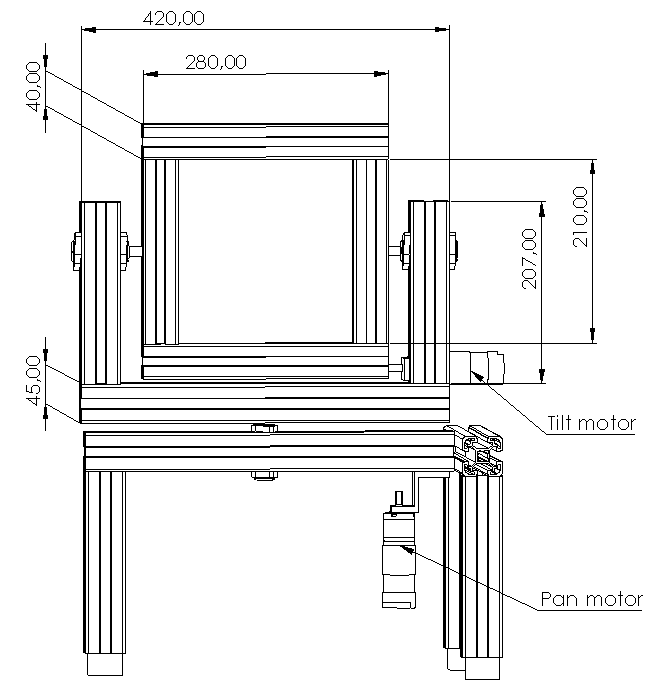
\includegraphics[width=0.5\textwidth]{Sections/Miscellaneous/Images/PhysicalMotorModel.png}
    \caption{Technical drawing of the pan-tilt system. All dimensions are in \SI{}{\milli \meter}.}
    \label{fig:Pan_Tilt_Drawing}
\end{figure}

% The project description states that the motor must be interfaced using an \textit{FPGA}, and that the motor control algorithms must be processed on the microcontroller. Each motor is fitted with an encoder that generates pulses as the motor turns, making it possible to determine the offset of the motor from a start position. The FPGA will be responsible for interfacing the encoders, as well as providing the \textit{PWM} signal controlling the voltage supplied to the motor. All communication between the two devices shall go through an \textit{SPI} connection in which the microcontroller is the master. The structure of the hardware implementation is provided in  and can be seen on the block diagram in figure \ref{fig:SystemOverviewIntroduction}.


\begin{figure}[H]
    \centering
    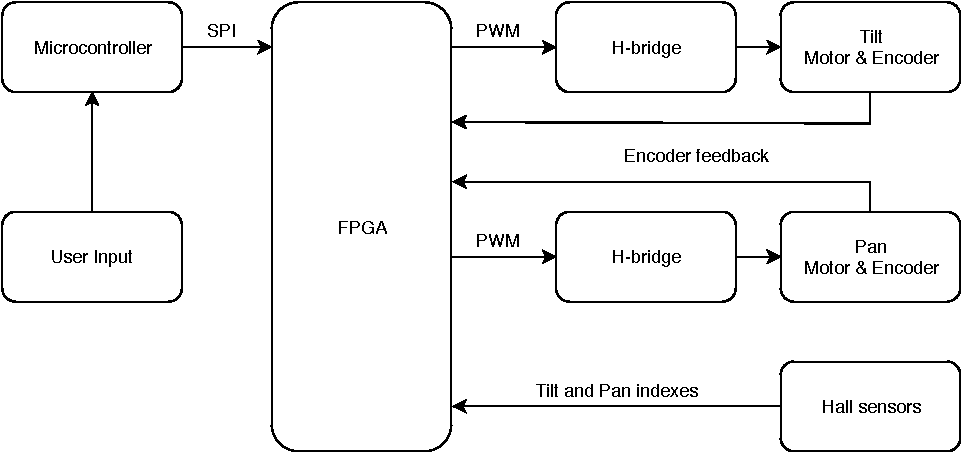
\includegraphics[width=0.7\textwidth]{Sections/Miscellaneous/Images/System_overview.pdf}
    \caption{Block diagram of the overall hardware structure.}
    \label{fig:SystemOverviewIntroduction}
\end{figure}

% To analyse the effect of different control algorithms and to find parameters needed for the control algorithms, a mathematical model of the pan-tilt system must be derived. This model will then be used to simulate the response of the control algorithm before implementing it on the pan-tilt system. However, the system introduces numerous different physical difficulties e.g. the friction, moment of inertia and limitations of the pan-tilt system. 

% Since the pan-tilt system is not to be dismantled, the physical parameters of the system are hard to determine, making it likely that differences between the modelling of the system and the physical system exists. 


% The goal of the project is to investigate different solutions for controlling the pan-tilt system, more than finding a specific controller configuration achieving a specified performance. 
% The project will mostly focus on classic control techniques, where both cascaded and single controller will be examined. While the primary focus will be on classic regulations techniques more modern ones will also be investigated for determine advantages and disadvantages.


% The purpose of the project is to design and control a \textit{pan-tilt system} as illustrated on figure \ref{fig:Pan_Tilt_Drawing}. The pan-tilt system is to take commands from a given medium of choice such as a computer. The controller must be implemented using both a microcontroller and a FPGA as illustrated on the block diagram on figure \ref{fig:SystemOverviewIntroduction}. The project specification states the controllers must be implemented on the microcontroller while the FPGA has to control the PWM supplied to the motors. All interchange of information between the two devices has to go through a SPI connection. The system is driven by two motors one for the pan and one for the tilt frame, which implies that a controller for each motor is to be designed. Furthermore the microcontroller is to manage user input to change the position of the robot.

% To design the controllers it is advantageous to model and simulate the system before implementing the controllers. However the system introduces numerous different physical difficulties e.g. the friction, moment of Inertia and limitations of the system. This renders a gab between the modelling of the system and the actual system, due to the fact that the actual physical parameters of the system are hard to measure and the pan-tilt system is not to be dismantled. A well-tuned controller can be the solution, minimizing the effect of the external noise and uncertainties. 

% Different solutions of controlling the motors are present e.g. having multiple controllers in cascade and different types of controllers. Wanting to implement multiple controllers in cascade controlling the position, velocity and the current, the physical behavior of the system is imperative to consider, due to the current being much faster relative to the position. Consideration which is crucial to have in mind when designing the controller. Using classic control techniques such as the PID-controller a relatively intuitive controller is introduced, making tuning of the system easier, but other means are possible such as modern control using state feedback or LQR. 

% The goal of this project is to design a controller which can reach a given position with a desired rise time, settling time and overshoot. This is to be achieved while examining different approaches to tune the controllers and different constellation of the controllers. 


%-what is the goal?
%-physical limitations/description
%-challenges
%-objective
%-introduce different solutions
\end{document}


